\documentclass[a4paper]{article}
\linespread{1.6}
\usepackage{geometry}
\usepackage{setspace}
\usepackage{amsmath}
\usepackage{amssymb}
\usepackage{enumerate}
\usepackage{subfigure}
\usepackage{caption}
\usepackage{listings}
\captionsetup{font = footnotesize}
\usepackage[pdftex]{graphicx}
\geometry{left=1cm,right=1cm,top=2.5cm,bottom=2.5cm}

\begin{document}
\begin{spacing}{2.0}
\begin{flushleft}\begin{huge}EEE6561  Fundamentals of Biometric Identification   Homework 2\end{huge}
\end{flushleft}
\begin{flushright}\begin{Large}Hudanyun Sheng\end{Large}\end{flushright}
\section*{\huge\textbf{ Part \uppercase\expandafter{\romannumeral1} Identity System Evaluation}  }
	\normalsize
	\begin{enumerate}[(a)]
		\item \textbf{For each of the systems, plot the genuine and imposter score distributions.}\\
		For both of the system 1 and system 2, the genuine and imposter score distribution are shown in 		same graph as histograms of the score distributions with 100 bins for each of them, shown in the 		form of probability:
		\begin{figure}[h]
		\begin{minipage}[t]{0.5\linewidth}
		\centering
		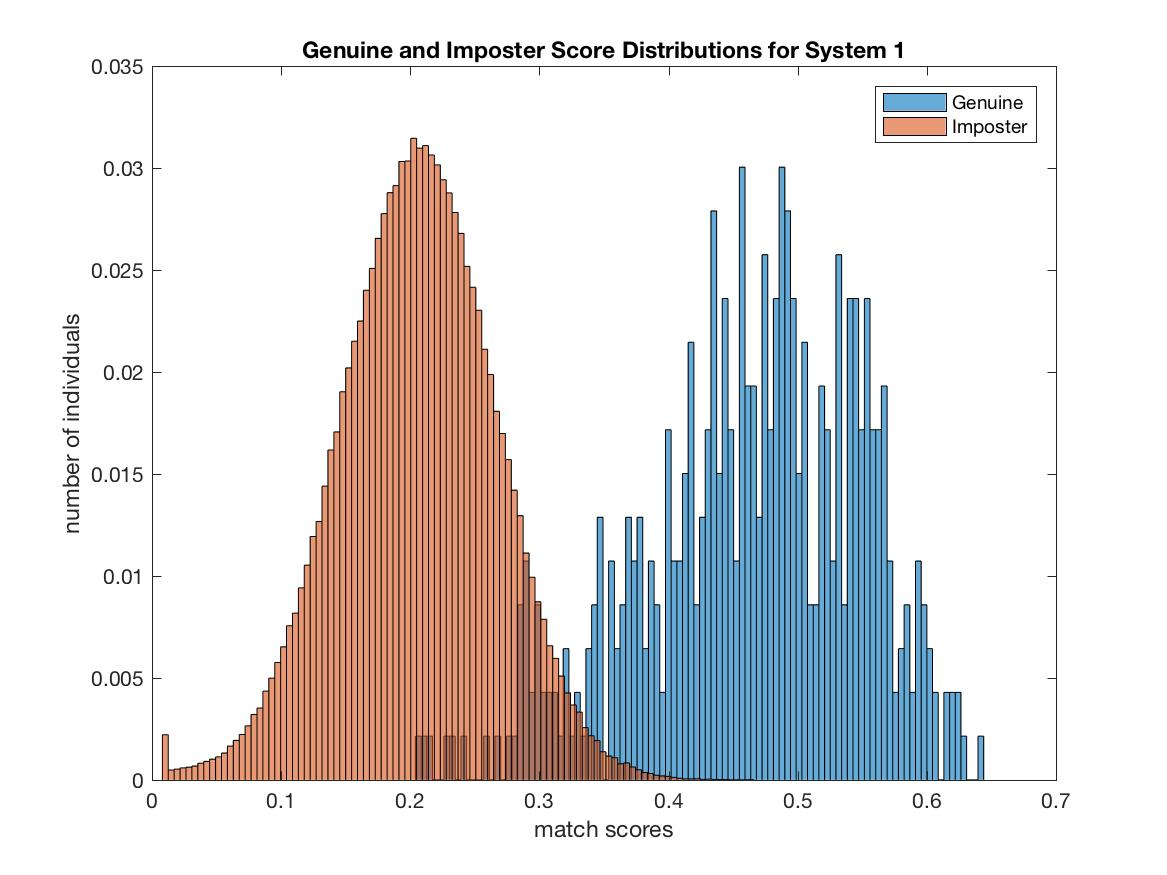
\includegraphics[width = 3.5in]{scoreDisSys1.jpg}
		\caption{Genuine and imposter score distributions for system 1}
		\end{minipage}
		\begin{minipage}[t]{0.5\linewidth}
		\centering
		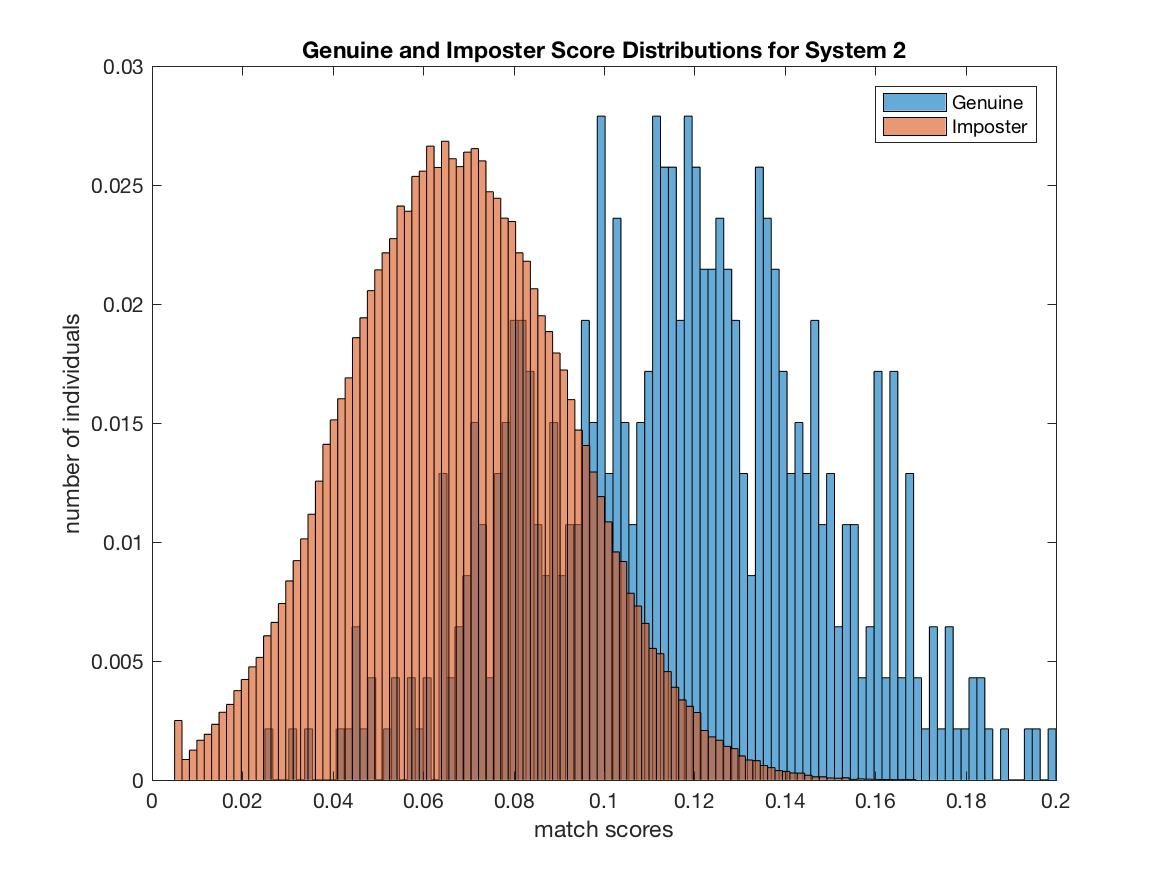
\includegraphics[width = 3.5in]{scoreDisSys2.jpg}
		\caption{Genuine and imposter score distributions for system 2}		
		\end{minipage}
		\end{figure}
		
		\item \textbf{For each of the systems, plot the Cumulative Match Characteristic curves.}\\
		For two systems, the cumulative match characteristic curves are shown in the same graph below, 		with rank from 1 to 200:
		\begin{figure}[h]
		\begin{minipage}[t]{0.5\linewidth}
		\centering
		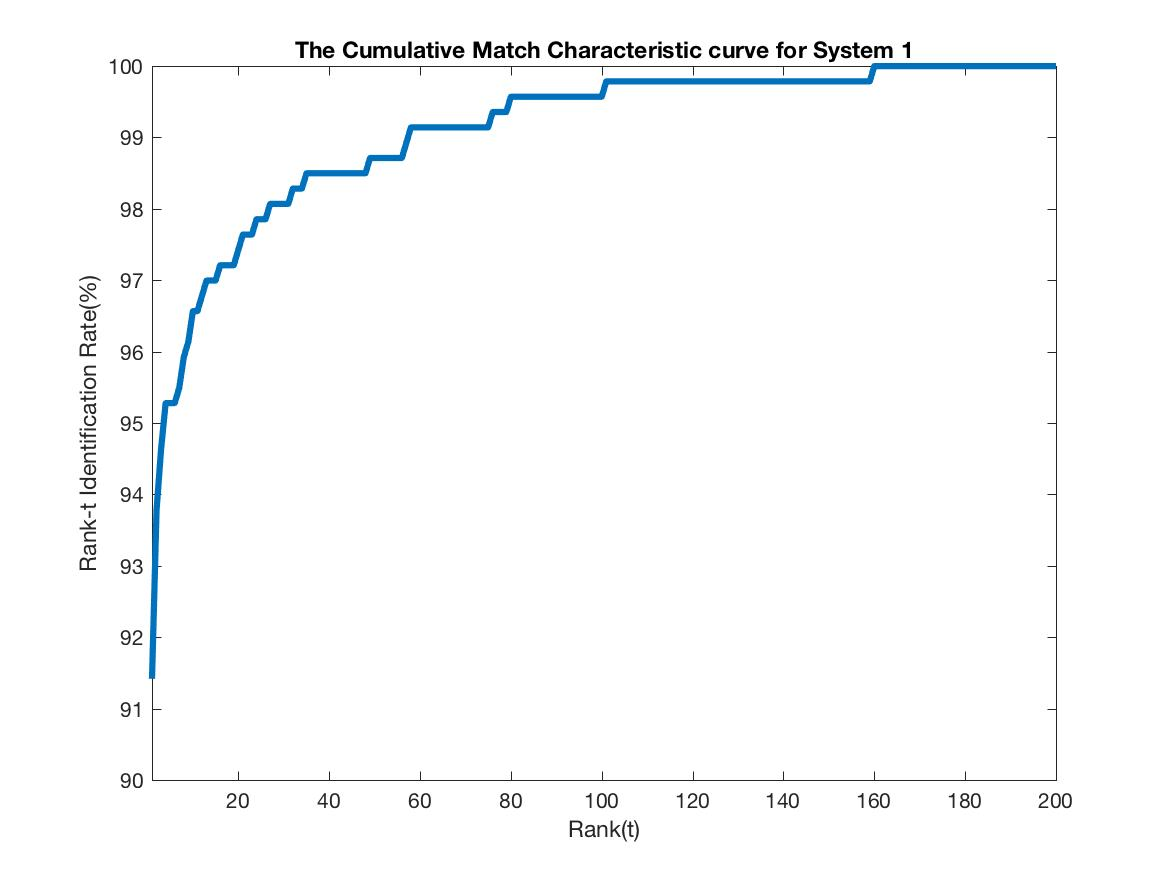
\includegraphics[width = 3.5in]{CMC1.jpg}
		\caption{The cumulative match characteristic curves for system 1.}
		\end{minipage}
		\begin{minipage}[t]{0.5\linewidth}
		\centering
		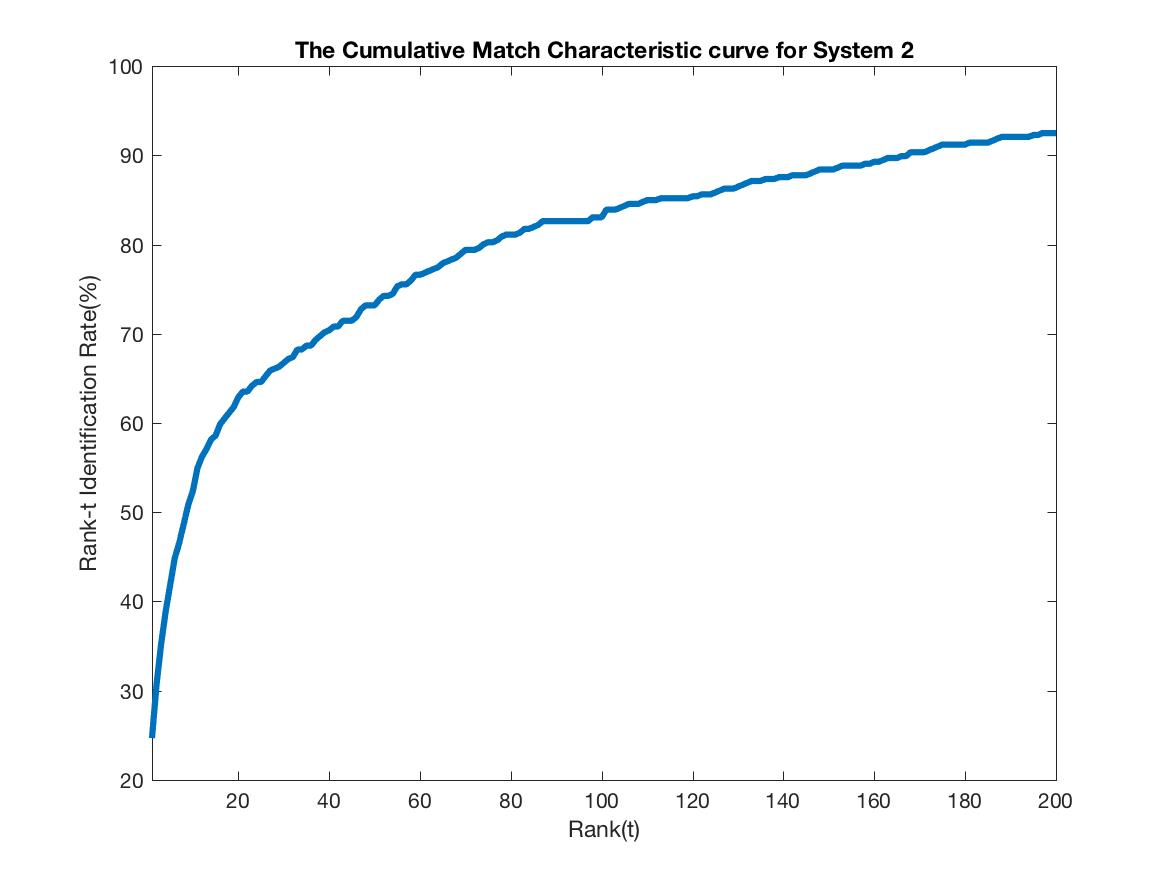
\includegraphics[width = 3.5in]{CMC2.jpg}
		\caption{The cumulative match characteristic curves for system 2.}
		\end{minipage}
		\end{figure}
		
		\item \textbf{For each of the systems, calculate the $d'$ (decidability index).}
		The d-prime value is defined as:
		$$d' = \displaystyle\frac{\sqrt{2}|\mu_1-\mu_0|}{\sqrt{\sigma_1^2+\sigma_0^2}}$$
		where $\mu_1(\mu_0)$ and $\sigma_1(\sigma_0)$ are the mean and standard deviation, 				respectively, of the genuine (imposter) score distributions.\\
		For system 1: $\mu_1 = 0.4639$, $\mu_0 = 0.2053$, $\sigma_1^2 = 0.0072$, $\sigma_0^2 = 			0.0036$, $d' = 3.5139$.\\
		For system 2: $\mu_1 = 0.1163$, $\mu_0 = 0.0679$,  $\sigma_1^2 = 0.0010$, $\sigma_0^2 = 			5.8172 \times 10^{-4}$, $d' = 1.7105$.
		
		\item \textbf{For each of the systems, what is the lowest rank at which the system achieves 				performance greater than $70\%$}.\\
		As shown in the figure below, we can conclude that system 1 achieves performance greater than 		$70\%$, which is, over $90\%$ at rank 1, while system 2 achieves performance greater than $70\%		$ only at rank 39 or greater.
		\begin{figure}[h]
		\centering
		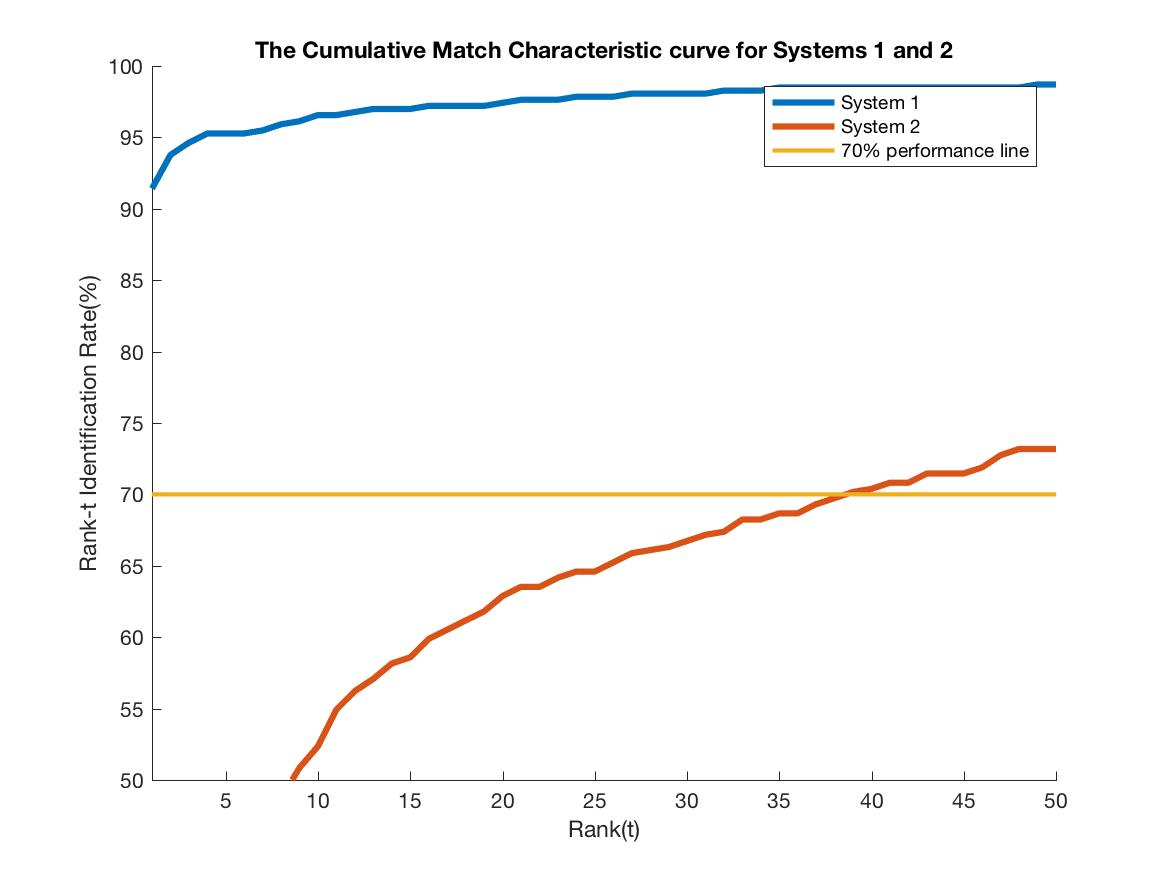
\includegraphics[width = 3.5in]{CMCwithLine.jpg}
		\caption{The cumulative match characteristic curves for both systems with a $70\%$ performance line.}
		\end{figure}
	\end{enumerate}

\newpage	
\section*{\huge\textbf{ Part \uppercase\expandafter{\romannumeral2} Verification System Evaluation}  }
	\normalsize
	\begin{enumerate}[(a)]
	\setcounter{enumi}{4}
	\item \textbf{For each of the systems, plot the Receiver Operating Curve (FAR vs. FRR).}\\
	The ROC curves for both of the systems are shown below in figure \ref{ROC}. 
	\begin{figure}[h]
	\centering
	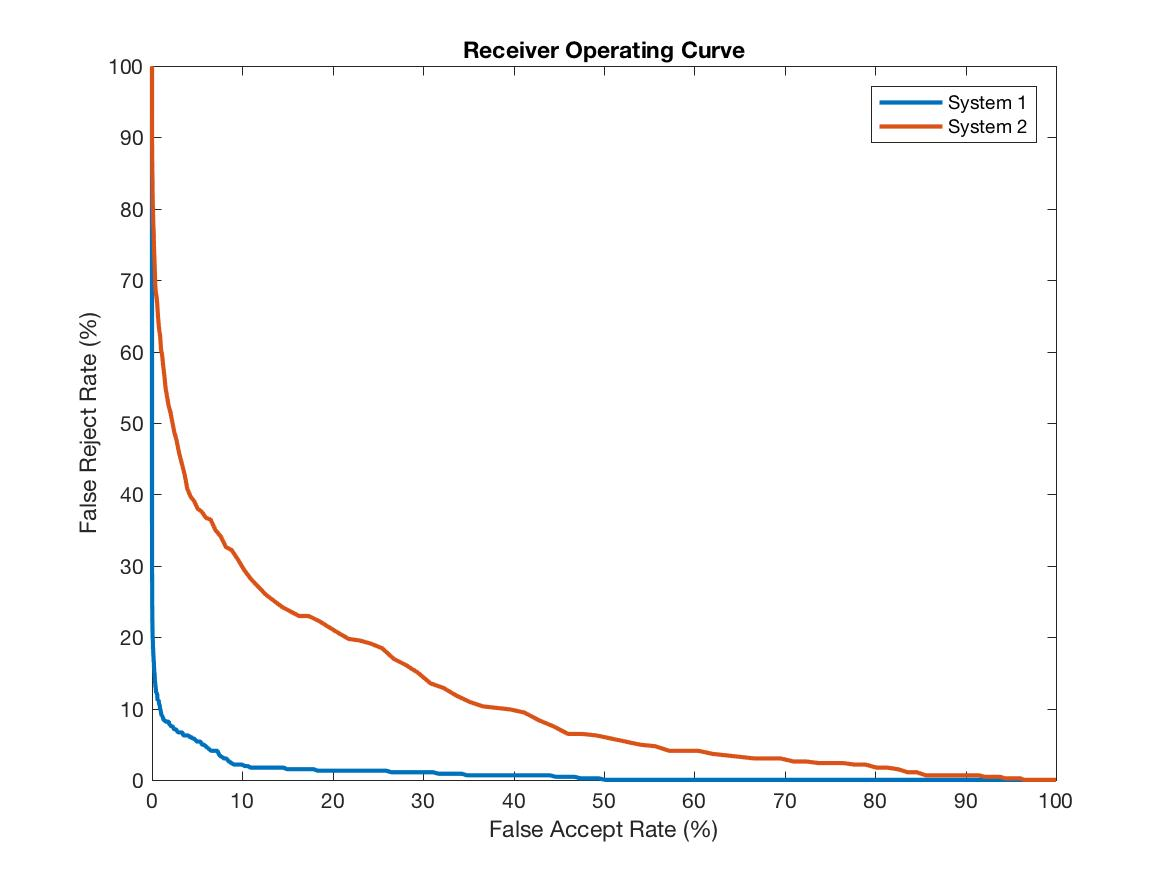
\includegraphics[width = 3.5in]{ROC.jpg}
	\caption{The receiver operating curves for systems 1 and 2.}
	\label{ROC}
	\end{figure}
	
	\item \textbf{For each of the systems, calculate the Equal Error Rate. At what operating point is this rate 		achieved for each system?}\\
	The plot of the equal error rate for both of the systems are shown in figure \ref{EER1} and \ref{EER2} below:
	\begin{figure}[h]
	\begin{minipage}[t]{0.5\linewidth}
	\centering
	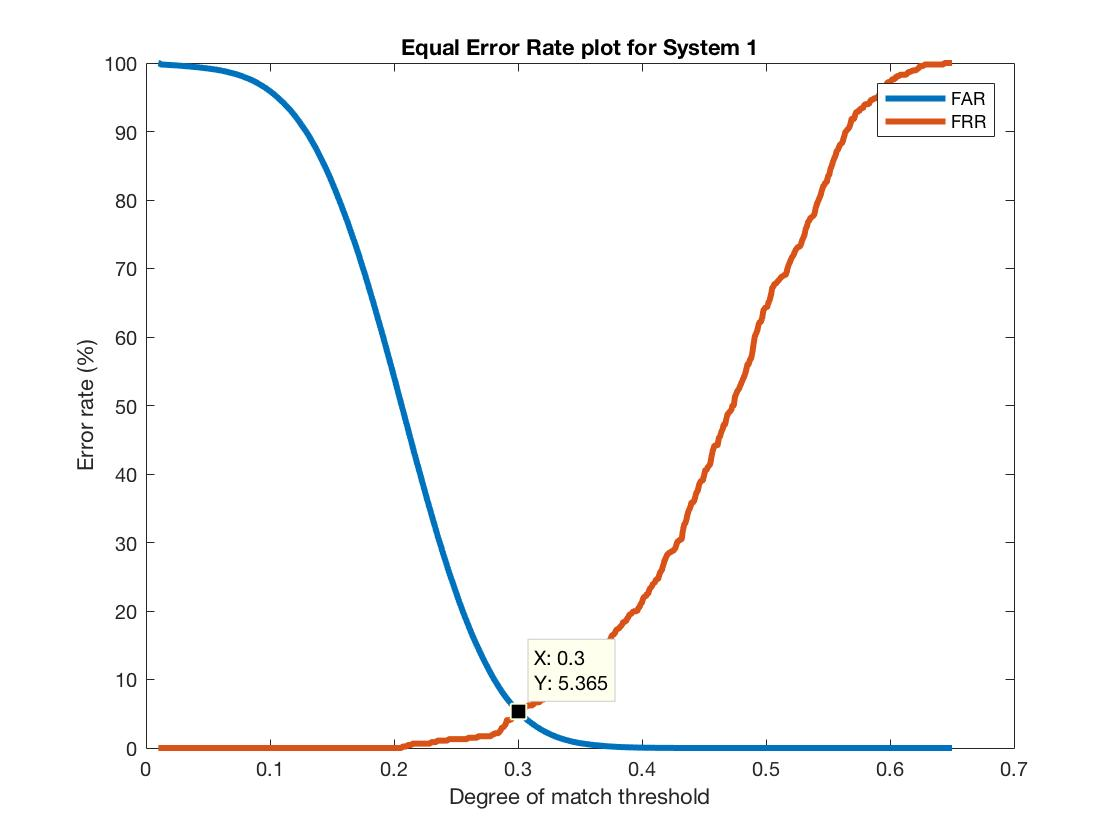
\includegraphics[width = 3.5in]{EER1.jpg}
	\caption{The plot of equal error rate for system 1.}
	\label{EER1}
	\end{minipage}
	\begin{minipage}[t]{0.5\linewidth}
	\centering
	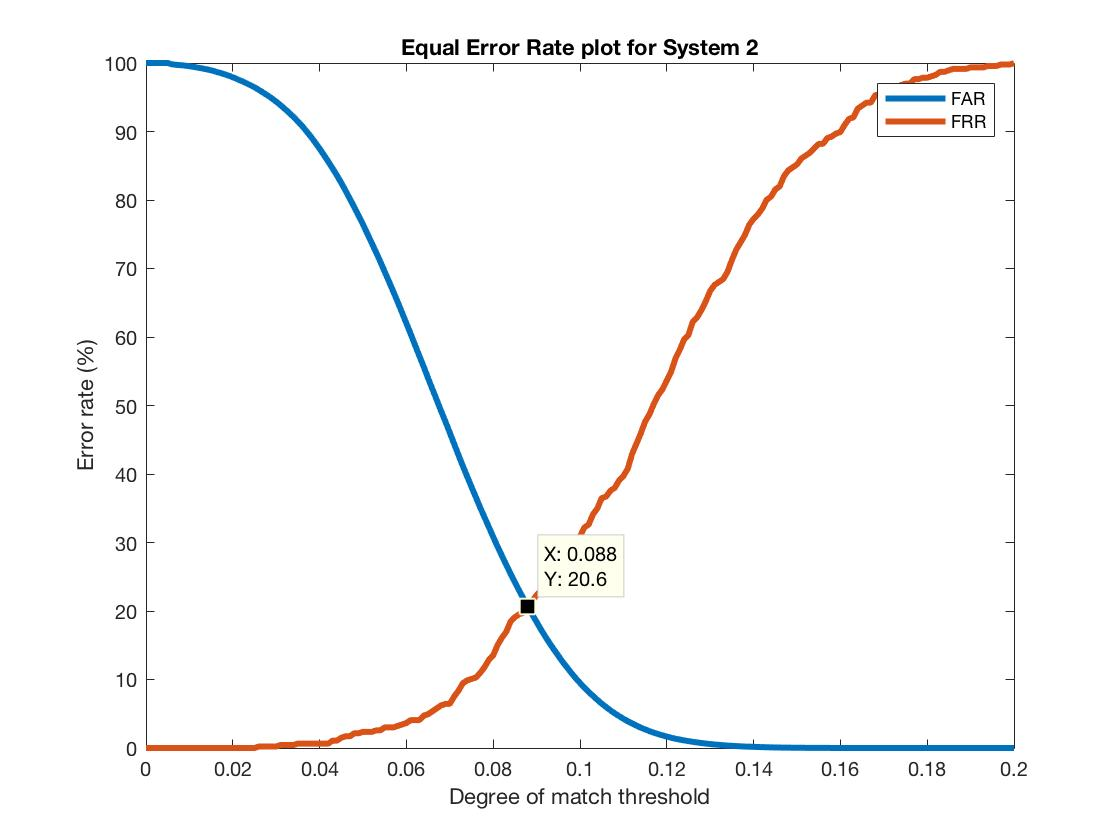
\includegraphics[width = 3.5in]{EER2.jpg}
	\caption{The plot of equal error rate for system 2.}
	\label{EER2}
	\end{minipage}
	\end{figure}
	By setting the some threshold, and conclude the FAR$=$FRR when the difference between FAR and FRR begin smaller than the threshold, which is the equal error rate. For \textbf{system 1}, with the threshold set to be 0.00001, the unique equal error rate is \textbf{5.365\%}; for \textbf{system 2}, with the threshold set to be 0.00005, the unique equal error rate is \textbf{20.6\%}. Which can also be easily learned from the plots. For system 1, the operating point to achieve the equal error rate is 0.3, for system 2, the operating point to achieve the equal error rate is 0.088.
	
	\item \textbf{For each of the systems, determine what the FRR is when the FAR $=1\%$, FAR $=5\%$, FAR $=10\%$, FAR $=20\%$. Present results in tabular format.}
	\begin{table}[h]
	\centering
	\begin{tabular}{|l|c|c|c|c|}
	\hline
	FAR & 1\% & 5\% & 10\% & 20\%\\
	\hline
	FRR of system 1 & 9.45\% & 5.36\% & 2.15\% & 1.29\%\\
	\hline
	FRR of system 2 & 60.3\% & 38.54\% & 30.18\% & 21.00\%\\
	\hline
	\end{tabular}
	\end{table}
	
	\item  \textbf{Which of the systems would you consider the best performing? Explain how you came to 	this determination.}\\
	Base on the discussions above, system 1 would perform better. Consider the score distribution for 		system 1, the score distribution for genuine scores and imposter scores are much more separated 		compared to system 2, whose scores for genuine and imposter have much overlap, which would make it hard to distinguish between them. Consider the cumulative match characteristic curve for both of the systems, we can see that the identification rate for system 1 starts at a much larger value than system 2, and increase with a higher rate. As discussed in part (d), the lowest rank for system 1 to achieve performance greater than $70\%$ is 1; while the lowest rank for system 2 to achieve performance greater than $70\%$ is 39. What is more, system 1 will reach identification rate of $100\%$ eventually; while system 2 will never reach identification rate of $100\%$. As discussed in part (c), the d'value for system 1 is larger than that for system 2. As is known to all, a larger d' value implies a better performance. When examine the ROC curves for both of the systems, the ROC curve for system 1 is much more closer to the axis, which implies better performance for the system. Also when considering the equal error rate, system 1 has the equal error rate of 5.365\%, while system 2 has the equal error rate of 20.6\% which is much larger than system 1's. As we know, systems with a lower EER is preferred. By comparing all these aspects,  the conclusion leads to that system 1 would I consider the best performing.
	\end{enumerate}
	
	\newpage
	\large{Attached are code for part \uppercase\expandafter{\romannumeral1} :}
	\normalsize
	\begin{lstlisting}
	clear; close all; clc
simMatrix{1} = importdata('simMatrix1.txt');
simMatrix{2} = importdata('simMatrix2.txt');
for idxSys = 1:2
    genuine{idxSys} = diag(simMatrix{idxSys});
    N{idxSys} = size(simMatrix{idxSys},1);
    mask1{idxSys} = eye(N{idxSys});
    mask2{idxSys} = ones(N{idxSys});
end
for idxSys = 1:2
    imposter{idxSys} = (mask2{idxSys}-mask1{idxSys}).*simMatrix{idxSys};
end

%% plot the genuine and imposter score distributions
for idxSys = 1:2
    temp = imposter{idxSys};
    temp(find(temp==0)) = [];
    figure, histogram(genuine{idxSys}, 100, 'Normalization', 'probability'), xlabel('match scores'), ylabel('number of individuals')
    hold on, histogram(temp, 100, 'Normalization', 'probability')
    title(['Genuine and Imposter Score Distributions for System ' num2str(idxSys)]), legend('Genuine', 'Imposter')
%     saveas(gcf, ['/Users/hudanyun.sheng/Google Drive/Me/201801Spring/EEE6561Fundamentals_of_BiometricIdentification/Homework/HW2/HW2_hudanyun_sheng/scoreDisSys' num2str(idxSys) '.jpg'])
end

%% plot the Cumulative Match Characteristic curves
n(1) = 200;
n(2) = 200;
y(1) = 90;
y(2) = 20;
for idxSys = 1:2
   sortedImposter{idxSys} = sort(imposter{idxSys}, 2, 'descend');
   for t = 1:n(idxSys)
       Rt{idxSys}(t) = length(find(sortedImposter{idxSys}(:,t)<genuine{idxSys}))/N{idxSys};
   end
   figure, plot(1:n(idxSys), Rt{idxSys}*100,  'Linewidth', 3), axis([1 n(idxSys) y(idxSys) 100]), xlabel('Rank(t)'), ylabel('Rank-t Identification Rate(%)'), title(['The Cumulative Match Characteristic curve for System ' num2str(idxSys)])
%    saveas(gcf, ['/Users/hudanyun.sheng/Google Drive/Me/201801Spring/EEE6561Fundamentals_of_BiometricIdentification/Homework/HW2/HW2_hudanyun_sheng/CMC' num2str(idxSys) '.jpg'])
end

%% calculate the d'
for idxSys = 1:2
	temp = imposter{idxSys};
    temp(find(temp==0)) = [];
    mu1{idxSys} = mean(genuine{idxSys});
    mu0{idxSys} = mean(temp);
    var1{idxSys} = var(genuine{idxSys}(:));
    var0{idxSys} = var(temp);
    
    d_prime{idxSys} = (sqrt(2)*abs(mu1{idxSys}-mu0{idxSys}))/sqrt(var1{idxSys}+var0{idxSys});
end


%% determine the lowest rank at which the systems achieve performance greater than 70%
n(1) = 50;
n(2) = 50;
y(1) = 50;
y(2) = 50;
figure
for idxSys = 1:2
   sortedImposter{idxSys} = sort(imposter{idxSys}, 2, 'descend');
   for t = 1:n(idxSys)
       Rt{idxSys}(t) = length(find(sortedImposter{idxSys}(:,t)<genuine{idxSys}))/N{idxSys};
   end
   hold on, plot(1:n(idxSys), Rt{idxSys}*100,  'Linewidth', 3), axis([1 n(idxSys) y(idxSys) 100]), xlabel('Rank(t)'), ylabel('Rank-t Identification Rate(%)')
end
hold on, plot(1:N{1}, 70*ones(1,N{1}), 'Linewidth', 2)
title('The Cumulative Match Characteristic curve for Systems 1 and 2')
legend('System 1', 'System 2', '70% performance line')
saveas(gcf, '/Users/hudanyun.sheng/Google Drive/Me/201801Spring/EEE6561Fundamentals_of_BiometricIdentification/Homework/HW2/HW2_hudanyun_sheng/CMCwithLine.jpg')
	\end{lstlisting}
	
	\newpage
	\large{Attached are code for part \uppercase\expandafter{\romannumeral2} }:
	\normalsize
	\begin{lstlisting}
	clear; close all; clc
simMatrix{1} = importdata('simMatrix1.txt');
simMatrix{2} = importdata('simMatrix2.txt');
for idxSys = 1:2
    genuine{idxSys} = diag(simMatrix{idxSys});
    N{idxSys} = size(simMatrix{idxSys},1);
    mask1{idxSys} = eye(N{idxSys});
    mask2{idxSys} = ones(N{idxSys});
end
for idxSys = 1:2
    imposter{idxSys} = (mask2{idxSys}-mask1{idxSys}).*simMatrix{idxSys};
end

%% plot the Receiver Operating Curve (FAR vs. FRR)
figure
for idxSys = 1:2
    temp = imposter{idxSys};
    temp(find(temp==0)) = [];
    eta_list{idxSys} = floor(min(temp)*100)/100:0.001:ceil(max(genuine{idxSys})*100)/100;
    for i = 1:length(eta_list{idxSys})
        eta = eta_list{idxSys}(i);
        FRR{idxSys}(i) = sum(genuine{idxSys}<eta)/length(genuine{idxSys});
        FAR{idxSys}(i) = sum(temp>eta)/length(temp);
    end
    plot(FAR{idxSys}*100, FRR{idxSys}*100, 'Linewidth', 2), hold on
end
xlabel('False Accept Rate (%)'), ylabel('False Reject Rate (%)'), title('Receiver Operating Curve' )
legend('System 1', 'System 2')
% saveas(gcf, '/Users/hudanyun.sheng/Google Drive/Me/201801Spring/EEE6561Fundamentals_of_BiometricIdentification/Homework/HW2/HW2_hudanyun_sheng/ROC.jpg')


%% calculate the Equal Error Rate
% thres = 0.00005;
for idxSys = 1:2
    figure, plot(eta_list{idxSys}, FAR{idxSys}*100, 'Linewidth', 3), hold on, plot(eta_list{idxSys}, FRR{idxSys}*100, 'Linewidth', 3)
    xlabel('Degree of match threshold'), ylabel('Error rate (%)'), legend('FAR', 'FRR')
    title(['Equal Error Rate plot for System ' num2str(idxSys)])
%     saveas(gcf, ['/Users/hudanyun.sheng/Google Drive/Me/201801Spring/EEE6561Fundamentals_of_BiometricIdentification/Homework/HW2/HW2_hudanyun_sheng/EER' num2str(idxSys) '.jpg'])
%     te{idxSys} = find(abs(FAR{idxSys}-FRR{idxSys})<thres);
end

idx = [28996 8800];
for idxSys = 1:2
    EER(idxSys) = FAR{idxSys}(idx(idxSys));
end

%%
for idxSys = 1:2
    sys{idxSys} = [FAR{idxSys};FRR{idxSys}];
end
	\end{lstlisting}

	
\end{spacing}
\end{document}